% ---
% Este capítulo, apresenta os conceitos sobre o algoritmo genético
% ---

\chapter{Implementação do algoritmo genético}
\label{chap:implementGA}

Para implementação do algoritmo foi utilizado a linguagem de programação JAVA de forma a aproveitar o paradigma de orientação a objetos com a característica de reaproveitamento de código. A estrutura do programa permite com classes básicas formar a lógica do algoritmo e com classes derivadas especializar o algoritmo para especificações de cada problema. Dessa forma com pouco código extra sendo feito é possível reaproveitar as classes já definidas, e usando o polimorfismo inerente a linguagens OO, é possível reescrever e acrescentar as partes necessárias para embutir conhecimento específico no problema.

\section{Implementação inicial}
Os testes começam sobre um modelo simples usando codificação binária para representar duas variáveis reais \textit{x} e \textit{y} com valores no intervalo \([-100,100]\), e 15 bits de comprimento. A conversão é feita usando um fator \textit{C} definido por \(C = \dfrac{200}{2^{15} - 1}\) que multiplicado pela representação binária transformada para o inteiro \textit{i} e somado ao valor mínimo, apresenta o valor real da variável, com resolução definida pelo fator,
\(x = C \cdot i_x - 100\). O cromossomo é formado por uma sequência de 30 bits, 15 para cada variável, concatenados na forma de um vetor (Em Java será utilizado os conceitos de Listas por serem mais versáteis com relação aos elementos que podem ser guardados e manipulados). A função que deve ser maximizada, que será a mesma de avaliação, é dada pela equação seguinte e apresenta o gráfico visto na \autoref{fig:grafico_teste1}: 
\[f(x,y) = \left| x \cdot y \cdot \sin\left(\frac{\pi \cdot y}{4}\right) \right|\] 
É possível ver que a função possui 4 pontos máximos definidos dentro do domínio, e utilizando o R para encontrar o máximo da função em um desses pontos, foi obtido os seguintes resultados: \(x = 100\), \(y = 98,01654\) e \(f(x,y) = 9800,827\). O ponto com é critico de ser encontrado pelo fato de possuir vários máximos locais dentro do domínio. Para comparação dos resultados do GA, sempre será executado uma busca aleatório com a quantidade de pontos gerados equivalentes a \(P * T\), onde \textit{P} é o tamanho da população definido como parâmetro do GA e \textit{T} o total de gerações que o algoritmo será executado.

%\begin{figure}[ht]
%	\centering
%	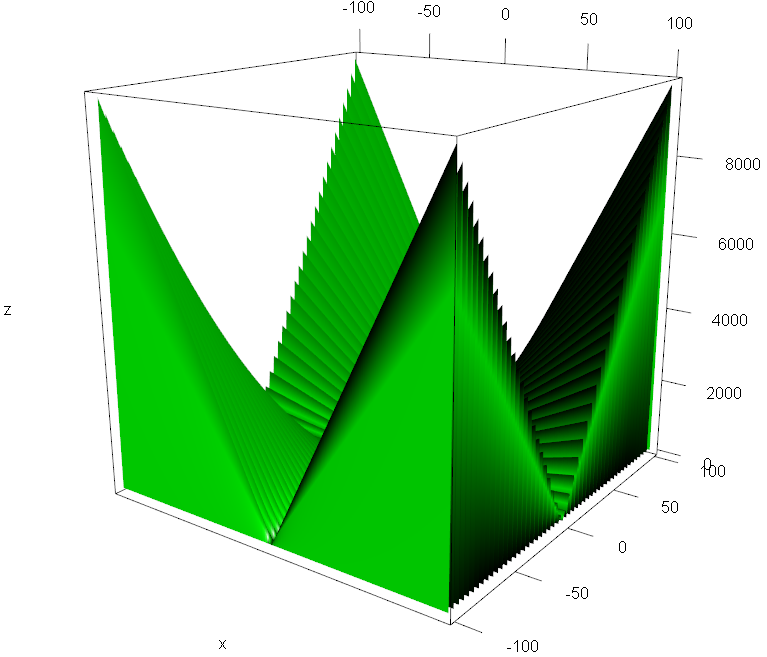
\includegraphics[width=1.1\linewidth]{imagens/teste1.png}
%	\caption{Gráfico da função de avaliação}
%	\label{fig:grafico_teste1}
%\end{figure}

\begin{figure}[ht]
	\centering
	\begin{subfigure}[b]{0.47\linewidth}
		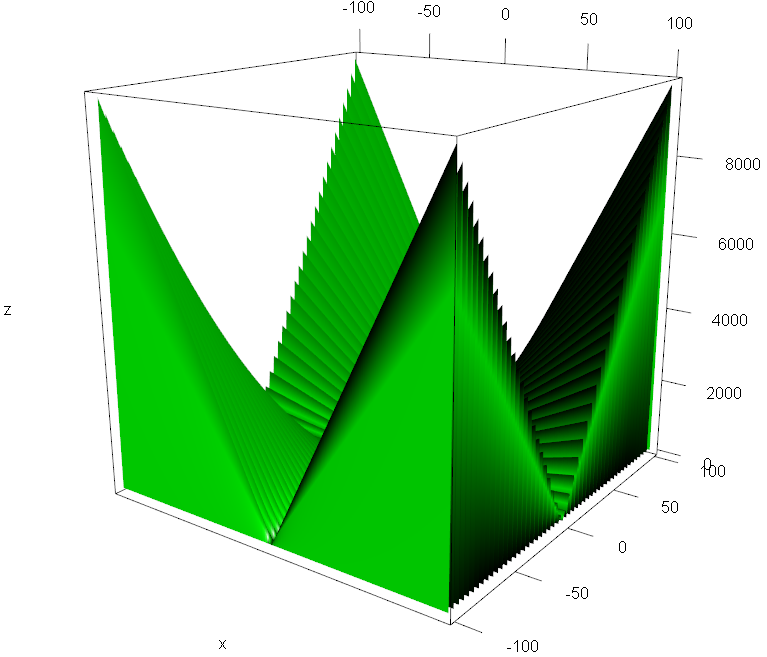
\includegraphics[width=\linewidth]{imagens/teste1.png}
		\caption{Gráfico no domínio completo}
	\end{subfigure}
	\begin{subfigure}[b]{0.47\linewidth}
		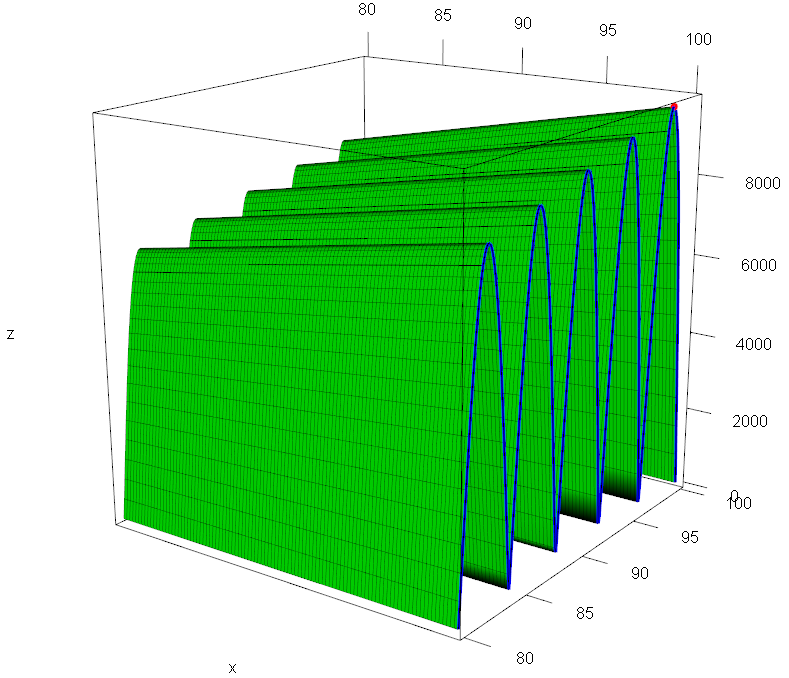
\includegraphics[width=\linewidth]{imagens/teste2.png}
		\caption{Gráfico ampliado em um dos máximos}
	\end{subfigure}
	\caption{Gráfico da função de avaliação}
	\label{fig:grafico_teste1}
\end{figure}

Para esse GA foi utilizado o método de seleção da roleta viciada, com um algoritmo simples que pode ser visto em \autoref{alg:roleta}, considerando a função \textit{random()} como um gerador de números aleatórios entre 0 e 1. Como pode ser visto, sorteia-se um número entre 0 e o valor da soma das avaliações da população, depois é feito um \textit{loop} iterando pelos valores das avaliações de cada cromossomo e somando a uma variável auxiliar. Ao atingir o valor sorteado, o ultimo individuo que teve seu valor somado a variável auxiliar é retornado.

\begin{algorithm}
	\LinesNumbered
	\Entrada{População de cromossomos: populacao}
	\Saida{Cromossomo selecionado: cromossomo}
	valor = random() * somaAvaliacao(populacao)\;
	aux = 0\;
	i = 1\;
	\Enqto{aux < valor  {\normalfont \textbf{e}} i <= populacao.tamanho()} {
			aux = aux + calculaAvaliacao(populacao[i])\;
			i = i + 1\;
	}
	\Retorna{populacao[i-1]}
	\caption{Roleta viciada}
	\label{alg:roleta}
\end{algorithm}

O operador de crossover testado foi o com único ponto de corte, e seu algoritmo pode ser visto em \autoref{alg:crossover}. O operador de mutação é feito apenas invertendo o estado do bit caso o sorteio seja positivo para aquele bit, respeitando o parâmetro de probabilidade de mutação. O critério de parada ficou definido apenas pela quantidade de iterações, isto é, quantas gerações da população foram produzidas. Para a população inicial são gerados cromossomos com bits aleatórios, sendo que é feito um sorteio individual para cada bit. Essa mesma operação é usada para gerar os valores para a busca randômica. Nesse primeiro teste a população é toda substituída por uma nova a cada geração, mas o melhor cromossomos de todas as gerações é guardado e apresentado como resultado final do algoritmo genético.

\begin{algorithm}
	\LinesNumbered
	\Entrada{Cromossomos: PaiA e PaiB; probabilidade de crossover: $p_c$}
	\Saida{Cromossomo Filho}
	\eSe{random() <= $p_c$}{
		corte = random() * PaiA.tamanho()\;
		\eSe{random() <= 0.5}{
			Filho = concatenar(PaiA[0:corte], PaiB[corte:PaiB.tamanho()])\;
		}{
			Filho = concatenar(PaiB[0:corte], PaiA[corte:PaiA.tamanho()])\;
		}
	}{
		Filho = PaiA\;
	}
	\Retorna{Filho}
	\caption{Crossover com um ponto de corte}
	\label{alg:crossover}
\end{algorithm}

Seguem alguns resultados para execução do GA, com os parâmetros: \(P = 30\), \(T = 10\), \(p_c = 0,8\), \(p_m = 0,01\), onde \textit{P} é o tamanho da população, \textit{T} é por quantas gerações o GA irá evoluir, \(p_c\) e \(p_m\) as probabilidades de crossover e mutação. No \autoref{qd:resultado_reproducao_t1} temos o resultado dos operadores de seleção, crossover e mutação para um descendente. O \textit{``HERITAGE MAP''} mostra qual porção do cromossomo herdou do pai 1 ou 2 e o \textit{``MUTATE MAP''} representa os bits que sofreram mutação. Além disso demonstra quantas vezes cada pai foi selecionado para produzir a nova geração, e com esses dados foi possível verificar os funcionamentos básicos do algoritmo, correspondendo ao esperado. %Como usamos 15 bits em cada uma das variáveis, o espaço de soluções possíveis tem \(2^{15} \cdot 2^{15} = 1.073.741.824\), e no caso da busca randômica cobre cerca de \(3000 / 1.073.741.824‬\) do espaço.

\begin{quadro}
\caption{\label{qd:resultado_reproducao_t1}Resultado de um ciclo de seleção, crossover e mutação do teste preliminar}
\begin{verbatim}
Geração: 1 | Média Avaliação: 2847,450535
#### CHILD #####
ID: 31
Fenotipo: x = -13,91949 | y = -94,32356
Avaliação: 1270,770525
#### PARENT 1 #####
ID: 11
Fenotipo: x = -13,91949 | y = -19,02829
Avaliação: 183,079928
Selecionado 1 vezes, 0,03

#### PARENT 2 #####
ID: 13
Fenotipo: x = 38,99960 | y = -94,28694
Avaliação: 3584,173001
Selecionado 6 vezes, 0,20

### HERITAGE MAP ###
111111111111111111122222222222
### MUTATE MAP
000000000000000000000000000000
#### CHILD #####
\end{verbatim}
\end{quadro}

Na \autoref{tab:resultados_teste1} é feito um comparativo entre o GA e a busca randômica (RS), executados em 1000 testes e calculado médias com intervalo de confiança e qual proporção o GA teve melhor resultado que o RS. Pode ser verificado que com poucas gerações, o GA apresentou resultados melhores que o RS, aumentando a população para 50 \(P=50\) o GA teve ainda uma pequena melhora com relação ao RS, mas aumentando para 100 gerações (\(T=100\)) os resultados praticamente são similares considerando os intervalos de confiança, porém percebe-se que ambos começaram a apresentar média de resultados maiores, e o GA supera o RS em menor quantidade de testes. Isso deve ocorrer, primeiro pelo fato do GA já não conseguir pelos operadores normais, refinar a solução, e segundo pelo RS ter cada vez mais amostras e com isso melhorar seu resultado.

Os testes com os outros parâmetros do GA se mostraram significativos também, com \(P = 30\), \(T = 10\), \(p_c = 0,8\), \(p_m = 0,05\), o GA apresentou resultados ainda melhores, particularmente com \(T=100\), mostrou expressiva melhora com relação ao teste anterior e ao RS. Isso mostra a necessidade do operador de mutação para garantir a exploração (\textit{exploration}) do espaço de soluções. Os testes alterando \(p_c = 0,9\) apresentaram nenhum efeito prático para esse problema, e o destaque ficou na ultima linha da tabela, onde ao usar em conjunto os parâmetros que individualmente melhoraram os resultados, obteve-se soluções muito próximas da ótima e um desempenho bem superior à busca aleatória.

\begin{table}[h]
	\begin{tabular}{|l|l|l|l|l|l|l|l|l|}
		\hline
		\multicolumn{4}{|c|}{\textbf{Parâmetros}} & \multicolumn{2}{c|}{\textbf{Resultados GA}} & \multicolumn{2}{c|}{\textbf{Resultados RS}} & \multicolumn{1}{c|}{\textbf{\#}} \\ \hline
		\textbf{P}     & \textbf{T}      & $\bm{p_c}$   & $\bm{p_m}$   & \textbf{Média $\pm$ IC}            & \textbf{D.P.}       & \textbf{Média $\pm$ IC}              & \textbf{D.P.}           & \textbf{GA $>$ RS}                                                               \\ \hline
		30    & 10     & 0,8	& 0,01    & 8693,10 $\pm$ 47,04     & 758,98    & 8419,40 $\pm$ 39,28       & 633,80        & 659                                                            \\ \hline
		50    & 10     & 0,8	& 0,01    & 9084,39 $\pm$ 32,39     & 522,60    & 8736,45 $\pm$ 32,43       & 523,22        & 716                                                            \\ \hline
		30    & 100    & 0,8	& 0,01    & 9369,35 $\pm$ 26,09     & 421,03    & 9352,98 $\pm$ 15,41       & 248,67        & 578                                                            \\ \hline
		30    & 10     & 0,8	& 0,05    & 8995,23 $\pm$ 35,40     & 571,19    & 8481,60 $\pm$ 38,72       & 624,75        & 741                                                            \\ \hline
		30    & 100    & 0,8	& 0,05    & 9670,58 $\pm$ 12,67     & 204,53    & 9367,58 $\pm$ 15,16       & 244,68        & 852                                                            \\ \hline
		30    & 10     & 0,9	& 0,01    & 8729,25 $\pm$ 45,65     & 736,59    & 8453,47 $\pm$ 39,33       & 634,68        & 623                                                            \\ \hline
		30    & 10     & 0,9	& 0,05    & 8997,06 $\pm$ 35,47     & 572,39    & 8504,56 $\pm$ 38,22       & 616,72        & 735                                                            \\ \hline
		50    & 100    & 0,8	& 0,05    & 9739,77 $\pm$ 8,45      & 136,34    & 9454,56 $\pm$ 12,07       & 194,75       & 927                                                            \\ \hline
	\end{tabular}
	\caption{Resultados teste simples com alguns parâmetros}
	\label{tab:resultados_teste1}
\end{table}

Além disso, pode ser vista a distribuição de um dos testes de busca aleatória, da ultima geração no GA e um comparativo da distribuição em algumas gerações \autoref{fig:scatter_RS_GA}. O ponto verde indica o melhor resultado para cada uma das distribuições. 
%\begin{figure}[ht]
%	\centering
%	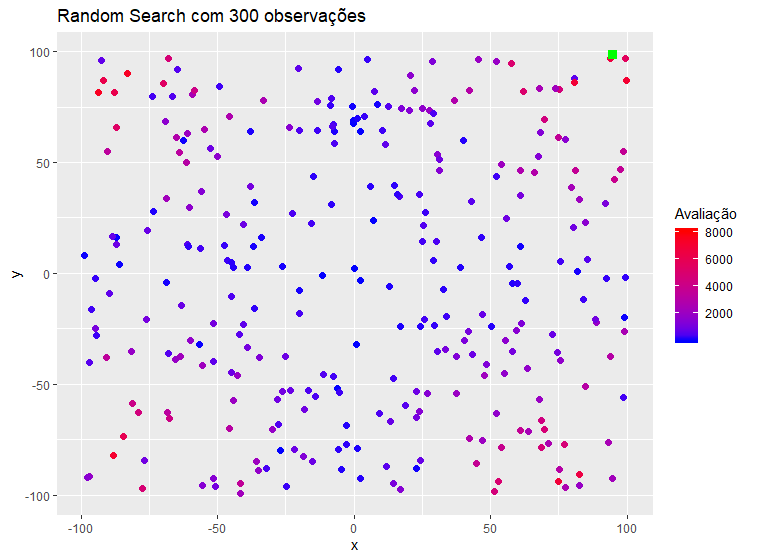
\includegraphics[width=0.8\linewidth]{imagens/scatter_rs_P30_T10.png}
%	\caption{Distribuição dos pontos na busca randômica (RS)}
%	\label{fig:scatter_RS}
%\end{figure}

\begin{figure}[ht]
	\centering
	\begin{subfigure}[b]{0.47\linewidth}
		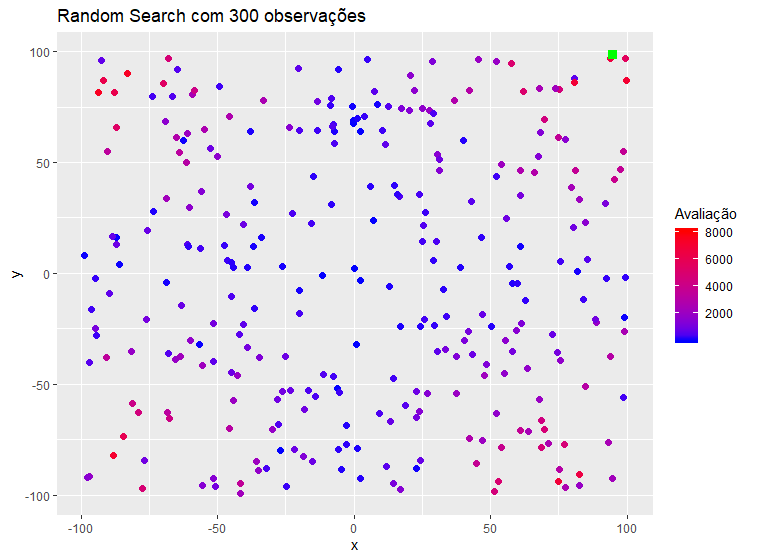
\includegraphics[width=\linewidth]{imagens/scatter_rs_P30_T10.png}
		\caption{Distribuição dos pontos gerados no RS}
	\end{subfigure}
	\begin{subfigure}[b]{0.47\linewidth}
		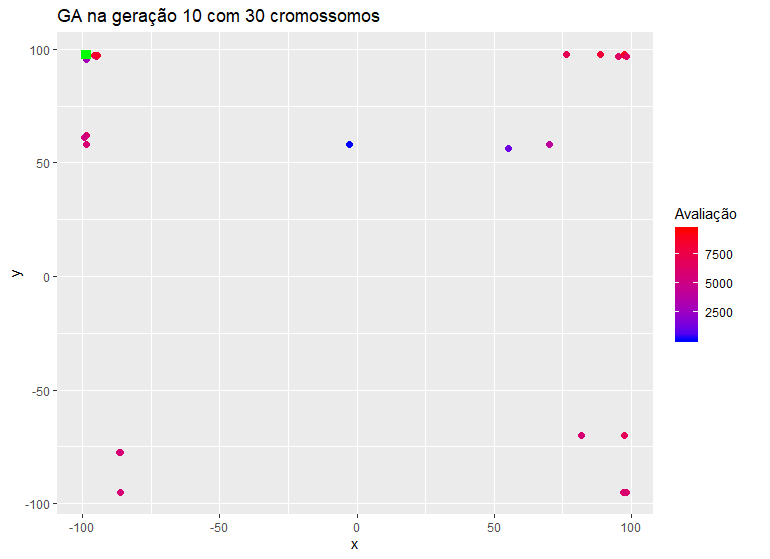
\includegraphics[width=\linewidth]{imagens/scatter_GA_P30_T10.png}
		\caption{Distribuição da ultima geração no GA}
	\end{subfigure}
	\begin{subfigure}[b]{0.65\linewidth}
		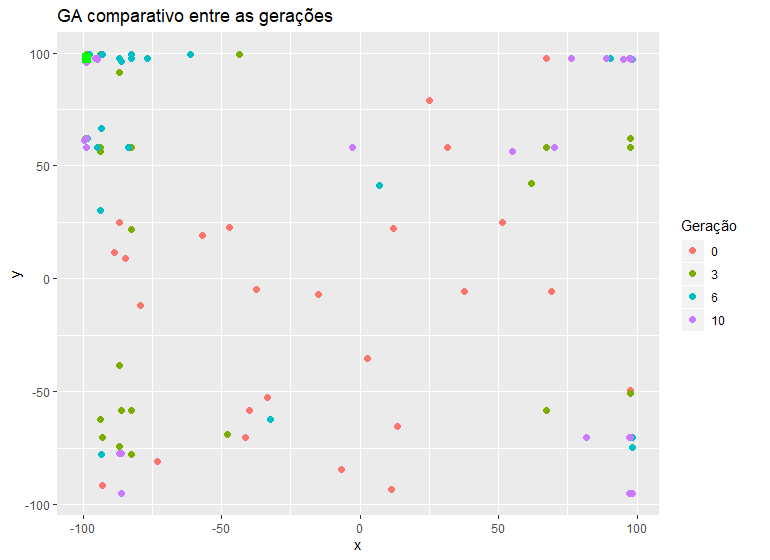
\includegraphics[width=\linewidth]{imagens/scatter_GA_P30_T10b.png}
		\caption{Comparativo entre algumas gerações do GA}
	\end{subfigure}
	\caption{Distribuições das soluções encontradas nos algoritmos de busca aleatória e GA}
	\label{fig:scatter_RS_GA}
\end{figure}



\section{Modelo de Ising}

O modelo de Ising\footnote{O modelo também é conhecido como Lenz-Ising, pois Lenz introduziu o modelo, porém nunca calculou nenhuma de suas propriedades} é um modelo da física para estudos de fênomenos magnéticos em materiais. Ising resolveu analiticamente o modelo para uma dimensão e depois Onsanger resolveu para uma rede quadrada (2D). Apesar do modelo ter sido elaborado para compreender melhor o propriedades magnéticas de certos materiais, ele se mostrou de grande utilidade para modelar problemas de outras áreas de estudos de fenômenos cooperativos, como por exemplo a dissertação de \citeonline{Lucena2014} onde usa o modelo de Ising aplicado a um estudo de criminalidade. É considerado um dos mais simples e estudado dos modelos de mecânica estatística.

O modelo define uma grade de \textit{spins} \(\sigma_t\) que podem conter os valores -1 e +1 somente. Esses spins possuem uma interação de energia dada por \(-J(t, t')\sigma_i\sigma_{t'}\), ou seja, o valor de energia de dois spins será \(-J(t, t')\) se os spins forem diferentes, e \(+J(t, t')\) se forem iguais, e adicionalmente podem interagir com um campo magnético externo \textit{H} com energia \(-H\sigma_t\). \cite{McCoy1973}.

Seja então \( \sigma_t \in \{ -1, +1 \} \) cada vértice do modelo, \(\Lambda\) representando a grade do modelo, e \(\Omega_{\Lambda} = \{-1, +1 \} ^ {\Lambda} \) o espaço de possíveis estados do modelo, define-se \(\sigma \in  \Omega_{\Lambda}\), \( \sigma = (\sigma_t)_{t \in \Lambda} \) como um estado possível do modelo de Ising para essas configurações. O Hamiltoniano do sistema para o estado \(\sigma\) (\(\mathcal{H}(\sigma)\)) será dado por: 

\[ \mathcal{H}(\sigma) = -\sum_{t,t' \in \Lambda}J(t,t')\sigma_{i}\sigma_{t'} -\sum_{t \in \Lambda}H \sigma_t \]

Sendo \(\beta = 1/kT\), com \textit{T} a temperatura em Kelvin e \textit{k} a constante de Boltzmann, a função de partição é definida por
\[ Z(\beta) = \sum_{\sigma \in \Omega_{\Lambda}} e^{-\beta \mathcal{H}(\sigma)} \]

e a probabilidade de encontrar o estado \(\sigma \)
\[ P(\sigma) = \frac{e^{-\beta \mathcal{H}(\sigma)}}{Z(\beta)} \]

Temperaturas altas deixam \(\beta\) baixo, o que torna a distribuição mais plana, e todos os estados tem probabilidades mais próximas de serem encontrados, conforme a temperatura baixa, os estados de menor energia passam a ter a maior probabilidade de ser encontrado.

O modelo de duas dimensões mais simples usa uma estrutura formada por quadrados com formato retangular de dimensões \(\Lambda = n \times m\), facilmente representada por uma matriz. Além disso \(J(t, t') = J_{tt'}\) é um valor fixo independente dos spins e que se \textit{t} e \textit{t'} não forem vizinhos será igual 0. Por fim será sem campo magnético externo, ou seja, \(H = 0\), e assim o Hamiltoniano pode ser reescrito na forma:

\begin{equation}
\mathcal{H}(\sigma) = - \sum_{i = 1}^{n-1} \sum_{j = 1}^{m-1} J_{tt'}\sigma_{i,j}\sigma_{i,j+1} + J_{tt'}\sigma_{i,j}\sigma_{i+1,j}
\label{eq:Energia_modelo_ising}
\end{equation}

O algoritmo genético simples será usado para apresentar uma solução, isto é \(\sigma\), para modelo de Ising em uma matriz \(10 \times 10\), com \(J_{tt'} = 1\) para os spins vizinhos, sendo \(\Lambda = \left[1,10\right]^2\) as posições da matriz, e a função de avaliação utilizada será baseada na \autoref{eq:Energia_modelo_ising}.

\section{GA para o modelo de Ising}
A classe cromossomo será usada para representar cada solução para o problema e conterá um vetor de valores inteiros de tamanho $100$, representando assim a matriz \( 10 \times 10 \), alinhando uma linha da matriz na sequencia da outra no vetor. Assim o nosso genótipo é uma cadeia de inteiros, onde o fenótipo será a matriz correspondente quebrando o vetor em linhas de tamanho $10$.

Exemplo da relação genótipo x fenótipo para uma matriz \( 3 \times 3 \):
\begin{align*}
\text{cromossomo} &= \left[-1, 1, 1, 1, -1, 1, 1, 1, -1 \right]\\
\text{fenótipo} &= \begin{bmatrix}
-1 & 1 & 1 \\
1 & -1 & 1 \\
1 & 1 & -1
\end{bmatrix}
\end{align*}

Usando os conceitos de OO, os cromossomos são definidos como classes, encapsulando os genes, os métodos dos operadores genéticos de crossover e mutação, e os métodos para avaliação e classificação dos cromossomos quando necessário. Para outros tipos de verificação também guardou informações sobre os cromossomos pais.

Para o método de seleção foi usado o método da roleta viciada, definindo a proporção de seleção de cada estado presente na população relacionado diretamente a sua função de avaliação. A primeira função testada foi usando o resultado da \autoref{eq:Energia_modelo_ising} somando o valor de \(\min\limits_{\sigma \in \Omega_{\sigma}}(\mathcal{H}(\sigma))\) e multiplicando por \(-1\) para conter somente valores positivos. Essa função não mostrou bons resultados pois não houve muita pressão seletiva, pois cromossomos com melhores valores recebiam pouco ou nenhum destaque na fase de seleção, assim o algoritmo precisava de muitas gerações para começar um avanço em encontrar melhores soluções. Na literatura sobre GA é mencionado o fato da função de avaliação ser muito plana o algoritmo passa a ser menos eficiente, isso também ocorre com outros métodos de otimização, como por exemplo os que usam gradientes por aproximação numérica, pois em funções que mostram pouco crescimento, a aproximação pode falhar em indicar a direção de maior crescimento. Os resultados para a seleção de uma das gerações pode ser visto na \autoref{tab:resumo_GA_H} do \refanexo{chap:anexos} .Para corrigir isso foi adotada a função de avaliação \(e^{-\beta \mathcal{H}(\sigma)} \) o que leva a uma probabilidade de seleção do indivíduo definida por:

\begin{equation}
Pr(\sigma) = \frac{e^{-\beta \mathcal{H}(\sigma)}}{\sum_{\sigma \in \Phi_{\Lambda}}e^{-\beta \mathcal{H}(\sigma)}}
\label{eq:selecao_modelo_ising}
\end{equation}

Onde \(\Phi_{\Lambda} \in \Omega_{\Lambda} \) representa a população de estados daquela geração do algoritmo e o método de seleção é parecido com o apresentado como seleção de Boltzmann na \autoref{subsec:selecao}. O problema que deve ser definido um novo parâmetro para o algoritmo dado por \(\beta \), que como valor inicial será usado o 0,05. Os resultados foram muito melhores e podem ser verificados na \autoref{tab:resumo_GA_expH} do \refanexo{chap:anexos}.

O operador de crossover será testado com o método de ponto único, dois pontos e uniforme, e para o operador de mutação cada posição do gene será sorteado com a probabilidade \(p_m\) para ser eleito para alteração e depois cada estado possível, no caso dois \(\{ -1, +1\}\), será sorteado com probabilidades iguais para definir o novo estado do gene.

A população inicial é definida sorteando os \(\sigma_t\) de cada posição das matrizes de cada um dos indivíduos. O programa terá definido uma classe para a população que é responsável por criar a geração inicial aleatória, controlar aspectos sobre a geração como melhor e pior cromossomo e algumas estatísticas sobre a população como quantidade de indivíduos que sofreram mutação e crossover, entre outros. 

Da mesma forma que o teste inicial, serão testados algumas variações dos parâmetros do algoritmo e comparado com os resultados da busca aleatória. Além disso será verificado, assim como no mencionado em \citeonline{Mitchell1996} sobre o trabalho de \citeonline{Pruegel-Bennett1994}, as distribuições dos valores de \(\mathcal{H}(\sigma)\) para as gerações 0, 10, 20, 30 e 40 do GA, e calculando as estatísticas para média e variância da amostra de 1000 testes. De forma ampliar as comparações dos resultados finais, os dois algoritmos foram modificado para ordenar as populações, que no caso do GA é feito a cada geração.

O começo da \autoref{tab:resultados_teste2} demonstra os resultados mantendo-se os parâmetros fixo e alterando apenas o método usado no crossover, indicado pelo índice nos valores de \(p_c\), com 1 para ponto único, 2 para crossover em dois pontos e \textit{u} para uniforme. Todos são muitos superiores ao método RS, provavelmente em virtude do espaço de soluções ser dado por \(2^{10*10}\) e a quantidade de observações geradas para o método estar cobrir uma parte pequena do espaço. Comparando o resultado entre os 3 métodos de crossover, é possível pela média dos resultados verificar pequena melhora usando o método para 2 pontos e mais uma pequena melhora para o uniforme, mais visível nos testes com mais gerações. Isso pode ser explicado pela construção do genótipo do cromossomos, como cada linha da matriz está na sequência da outra, podemos ter \textit{clusters} com bom resultados de forma quadrada, como mostrado na \autoref{fig:Map_ising}. A região vermelha possui uma baixa energia contribuindo de forma positiva para a avaliação do indivíduo, porém essa área não consegue ser isolada pelos operadores de crossover de 1 ou 2 pontos, mas tem boa probabilidade de ser compartilhada em partes ou inteira através do operador uniforme. Outro fator que piora nessa condição é os genes caronistas, discutidos na \autoref{sec:problemas_GA}, pois a área azul ao apresentar pior resultado tem alta probabilidade de pegar carona com a área vermelha do cromossomo.

\begin{table}[htb]
	\centering
	\begin{tabular}{|l|l|l|l|l|l|l|l|l|}
		\hline
		\multicolumn{4}{|c|}{\textbf{Parâmetros}}                                                    & \multicolumn{2}{c|}{\textbf{Resultados GA}}                                        & \multicolumn{2}{c|}{\textbf{Resultados RS}}                                        & \multicolumn{1}{c|}{\textbf{\#}}                      \\ \hline
		\textbf{P} & \textbf{T} & $\bm{p_c}$ & $\bm{p_m}$ & \textbf{Média $\pm$ IC} & \textbf{D.P.} & \textbf{Média $\pm$ IC} & \textbf{D.P.} & \textbf{GA < RS} \\ \hline
	30                          & 10                          & $0,8_1$    & 0,02       & -58.90 $\pm$ 0,54                            & 8,77                           & -39,05 $\pm$ 0,33                            & 5,43                           & 978                                          \\ \hline
	30                          & 10                          & $0,8_2$    & 0,02       & -60,21 $\pm$ 0,57                            & 9,33                           & -38,98 $\pm$ 0,32                            & 5,22                           & 970                                          \\ \hline
	30                          & 10                          & $0,8_u$    & 0,02       & -60,42 $\pm$ 0,63                            & 10,30                          & -39,39 $\pm$ 0,35                            & 5,68                           & 960                                          \\ \hline
	30                          & 100                         & $0,8_1$    & 0,02       & -122,24 $\pm$ 0,71                           & 11,57                          & -48,54 $\pm$ 0,27                            & 4,49                           & 1000                                         \\ \hline
	30                          & 100                         & $0,8_2$    & 0,02       & -126,05 $\pm$ 0,75                           & 12,19                          & -47,94 $\pm$ 0,27                            & 4,48                           & 1000                                         \\ \hline
	30                          & 100                         & $0,8_u$    & 0,02       & -130,47 $\pm$ 0,73                           & 11,89                          & -48,23 $\pm$ 0,28                            & 4,54                           & 1000                                         \\ \hline
\end{tabular}
\caption{Resultados da média de energia para 1000 testes com modelo Ising alterando tipo de crossover}
\label{tab:resultados_teste2}
\end{table}

\begin{figure}[ht]
	\centering
	\includegraphics[width=0.5\linewidth]{imagens/Mapa_ising.png}
	\caption{Exemplo de uma região (vermelha) com baixa energia, próxima de outras com energias superiores}
	\label{fig:Map_ising}
\end{figure}

Nos próximos testes fica fixado o crossover uniforme, além disso pela característica do GA, quanto mais iterações do algoritmo permitida, melhores resultados deve apresentar, portanto serão avaliados os demais parâmetros temos os resultados apresentados na \autoref{tab:resultados_teste3}. Pelos valores de média apresentado é possível ver que os parâmetros \(p_c = 0,8\) e \(p_m = 0,02\), apresentaram os melhores resultados, quando o \(p_m\) é aumentado, como o algoritmo não tem elitismo, é provável que os melhores esquemas se perdem com a mutação. O \(p_c\) com valores mais baixos teve um resultado pior, que indica que com menos crossover deve ter ocorrido menos \textit{exploitation} do algoritmo levando a uma convergência mais lenta.

\begin{table}[htb]
	\centering
	\begin{tabular}{|l|l|l|l|l|l|l|l|l|}
		\hline
		\multicolumn{4}{|c|}{\textbf{Parâmetros}}                                                    & \multicolumn{2}{c|}{\textbf{Resultados GA}}                                        & \multicolumn{2}{c|}{\textbf{Resultados RS}}                                        & \multicolumn{1}{c|}{\textbf{\#}}                      \\ \hline
		\textbf{P} & \textbf{T} & $\bm{p_c}$ & $\bm{p_m}$ & \textbf{Média $\pm$ IC} & \textbf{D.P.} & \textbf{Média $\pm$ IC} & \textbf{D.P.} & \textbf{GA < RS} \\ \hline
		30                          & 40                          & 0,8        & 0,02       & -105,07 $\pm$ 0,72                           & 11,66                          & -44,98 $\pm$ 0,31                            & 5,01                           & 1000                                      \\ \hline
		30                          & 40                          & 0,8        & 0,05       & -93,90 $\pm$ 0,71                            & 11,52                          & -44,63 $\pm$ 0,29                            & 4,81                           & 1000                                      \\ \hline
		30                          & 40                          & 0,8        & 0,01       & -101,69 $\pm$ 0,74                           & 11,96                          & -44,91 $\pm$ 0,30                            & 4,85                           & 1000                                      \\ \hline
		40                          & 40                          & 0,8        & 0,02       & -111,06 $\pm$ 0,73                           & 11,89                          & -46,24 $\pm$ 0,30                            & 4,87                           & 1000                                      \\ \hline
		40                          & 40                          & 0,8        & 0,01       & -109,59 $\pm$ 0,73                           & 11,84                          & -46,02 $\pm$ 0,31                            & 5,04                           & 1000                                      \\ \hline
		30                          & 40                          & 0,95       & 0,02       & -108,42 $\pm$ 0,75                           & 12,15                          & -44,91 $\pm$ 0,31                            & 5,14                           & 1000                                      \\ \hline
		30                          & 40                          & 0,7        & 0,02       & -101,26 $\pm$ 0,69                           & 11,27                          & -44,78 $\pm$ 0,31                            & 5,10                           & 1000                                      \\ \hline
	\end{tabular}
	\caption{Resultados da média de energia para 1000 testes com modelo Ising alterando outros parâmetros}
	\label{tab:resultados_teste3}
\end{table}

Os resultados mostrados foram para o melhor cromossomo encontrado entre todas as gerações do GA. A \autoref{tab:resultados_teste4} mostra mais dois resultados para a implementação do elitismo mantendo os 3 melhores cromossomos para a próxima população. Os valores indicam que houve pequena melhora no algoritmo.

\begin{table}[htb]
	\centering
	\begin{tabular}{|l|l|l|l|l|l|l|l|l|}
		\hline
		\multicolumn{4}{|c|}{\textbf{Parâmetros}}                                                    & \multicolumn{2}{c|}{\textbf{Resultados GA}}                                        & \multicolumn{2}{c|}{\textbf{Resultados RS}}                                        & \multicolumn{1}{c|}{\textbf{\#}}                      \\ \hline
		\textbf{P} & \textbf{T} & $\bm{p_c}$ & $\bm{p_m}$ & \textbf{Média $\pm$ IC} & \textbf{D.P.} & \textbf{Média $\pm$ IC} & \textbf{D.P.} & \textbf{GA < RS} \\ \hline
		30                          & 40                          & 0,8        & 0,02       & -110,66 $\pm$ 0,66                           & 10,73                          & -44,81 $\pm$ 0,30                            & 5,88                           & 1000                                      \\ \hline
		30                          & 40                          & 0,95        & 0,02       & -113,69 $\pm$ 0,70                            & 11,36                          & -44,75 $\pm$ 0,30                            & 4,99                           & 1000                                      \\ \hline
	\end{tabular}
	\caption{Resultados da média de energia para 1000 testes com modelo Ising e usando elitismo mantendo 3 cromossomos}
	\label{tab:resultados_teste4}
\end{table}


Para completar as avaliações, mantendo os parâmetros \(P = 50\), \(T = 40\), \(p_c = 0,95\), \(p_m = 0,02\) e com elitismo mantendo 3 cromossomos, foram salvos os valores de energia da população dos 1000 testes para as gerações 0, 10, 20, 30 e 40. Depois foi calculado a média e variância dessas gerações para cada um dos testes e finalmente feita a média dos parâmetros entre os 1000 testes obtendo os valores mostrados na \autoref{tab:resultados_medias_var}

\begin{table}[htb]
	\centering
	\begin{tabular}{|l|c|c|c|c|c|}
		\hline
		\textbf{Geração}   & \textbf{0} & \textbf{10} & \textbf{20} & \textbf{30} & \textbf{40} \\ \hline
		\textbf{Média}     & 0,00       & -47,49      & -78,76      & -96,46      & -106,86      \\ \hline
		\textbf{Variância} & 178,55     & 158,42      & 117,09       & 106,79       & 103,55       \\ \hline
	\end{tabular}
	\caption{Resultados da média de energia para 1000 testes das gerações 0, 10, 20, 30 e 40 do modelo Ising e usando elitismo com 3 cromossomos}
	\label{tab:resultados_medias_var}
\end{table}

\begin{figure}[ht]
	\centering
	\begin{subfigure}[b]{0.47\linewidth}
		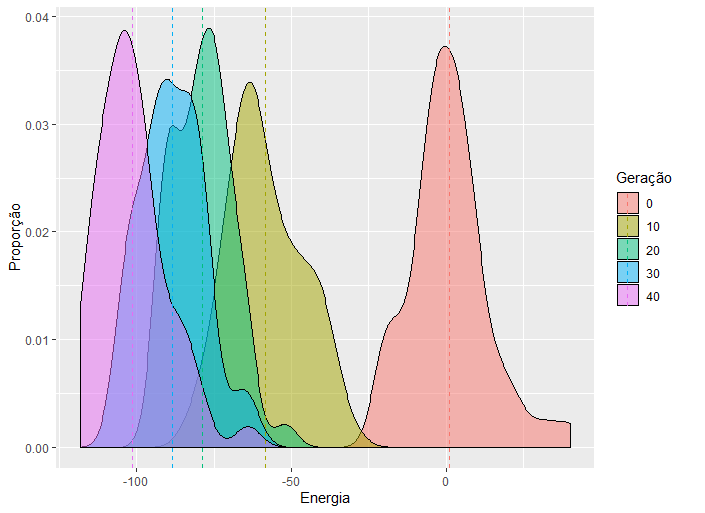
\includegraphics[width=\linewidth]{imagens/distribuicao_t50.png}
		\caption{Distribuição das amostras no teste 50}
	\end{subfigure}
	\begin{subfigure}[b]{0.47\linewidth}
		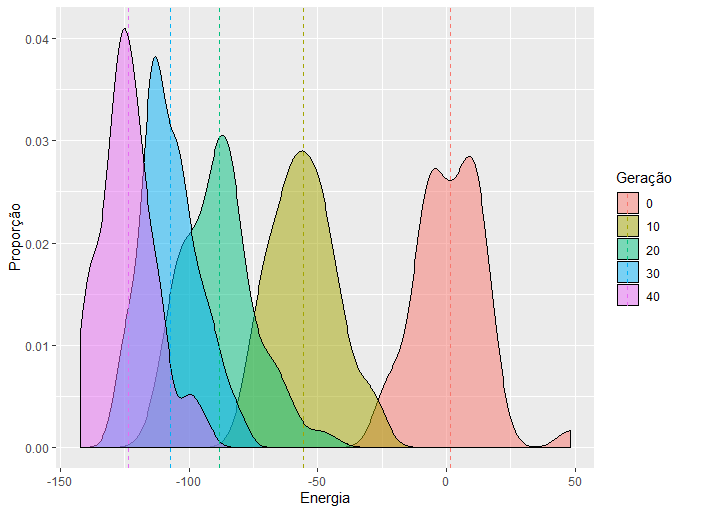
\includegraphics[width=\linewidth]{imagens/distribuicao_t491.png}
		\caption{Distribuição das amostras no teste 491}
	\end{subfigure}
	\begin{subfigure}[b]{0.47\linewidth}
		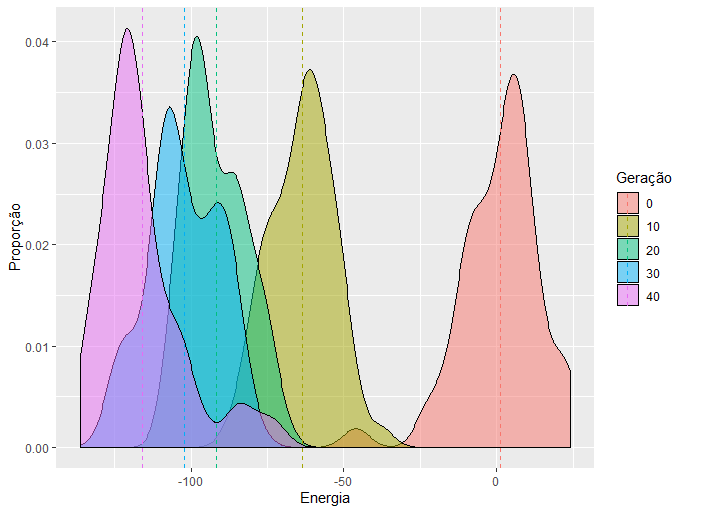
\includegraphics[width=\linewidth]{imagens/distribuicao_t900.png}
		\caption{Distribuição das amostras no teste 900}
	\end{subfigure}
	\begin{subfigure}[b]{0.47\linewidth}
		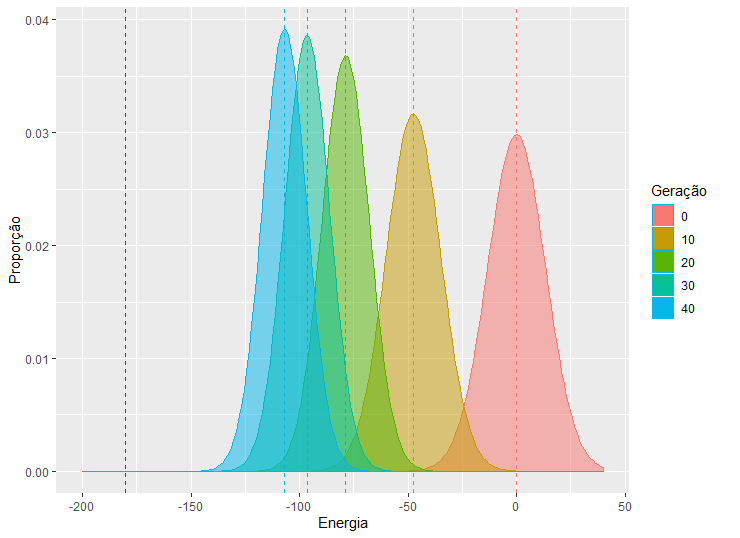
\includegraphics[width=\linewidth]{imagens/Distribuicao_medias.png}
		\caption{Usando média dos valores e considerando distribuição normal}
	\end{subfigure}
	\caption{Distribuições das populações para gerações 0, 10, 20 e 40, com \(p_m=0,02\)}
	\label{fig:distribuicao_ising_1}
\end{figure}

Diferente resultados vistos em \citeonline{Pruegel-Bennett1994}, a variância reduz pouco, o que é esperado, pois no teste proposto só foi usado o operador de crossover. Refazendo os testes com \(p_m = 0\) obtemos a seguinte \autoref{tab:resultados_medias_var2}. O operador de mutação mantém a variância na população pois ele garante o \textit{exploration}, mantendo a diversidade da população.

\begin{table}[htb]
	\centering
	\begin{tabular}{|l|c|c|c|c|c|}
		\hline
		\textbf{Geração}   & \textbf{0} & \textbf{10} & \textbf{20} & \textbf{30} & \textbf{40} \\ \hline
		\textbf{Média}     & -0,02       & -52,34      & -85,29      & -96,25      & -98,72      \\ \hline
		\textbf{Variância} & 180,96     & 120,07      & 36,62       & 8,01       & 1,54       \\ \hline
	\end{tabular}
	\caption{Resultados da média de energia para 1000 testes com modelo Ising usando elitismo mantendo 3 cromossomos}
	\label{tab:resultados_medias_var2}
\end{table}


\begin{figure}[ht]
	\centering
	\begin{subfigure}[b]{0.47\linewidth}
		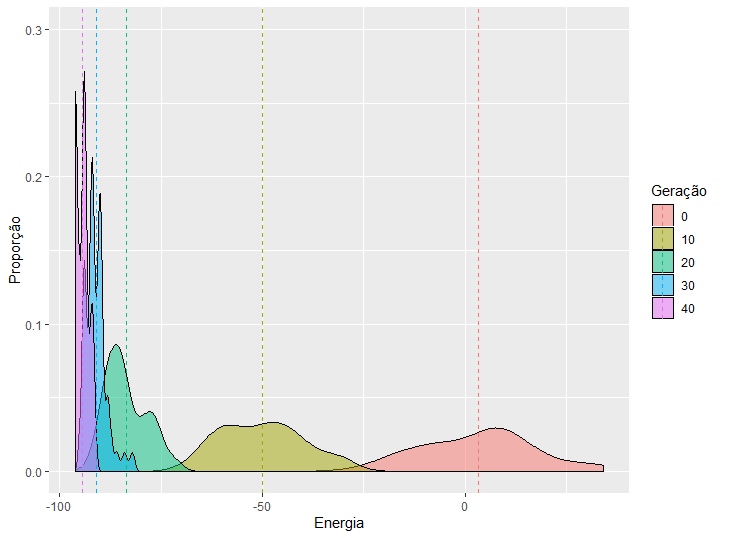
\includegraphics[width=\linewidth]{imagens/distribuicao_t43_2.png}
		\caption{Distribuição das amostras no teste 43}
	\end{subfigure}
	\begin{subfigure}[b]{0.47\linewidth}
		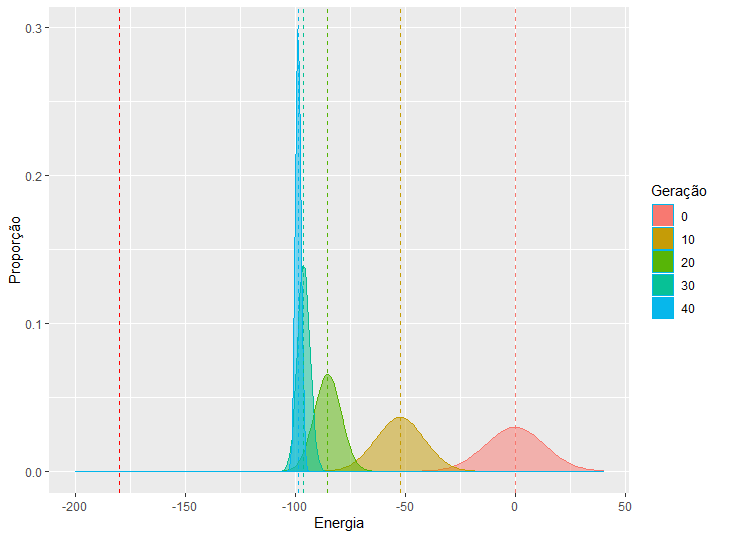
\includegraphics[width=\linewidth]{imagens/Distribuicao_medias2.png}
		\caption{Usando média dos valores e considerando distribuição normal}
	\end{subfigure}
	\begin{subfigure}[b]{0.67\linewidth}
		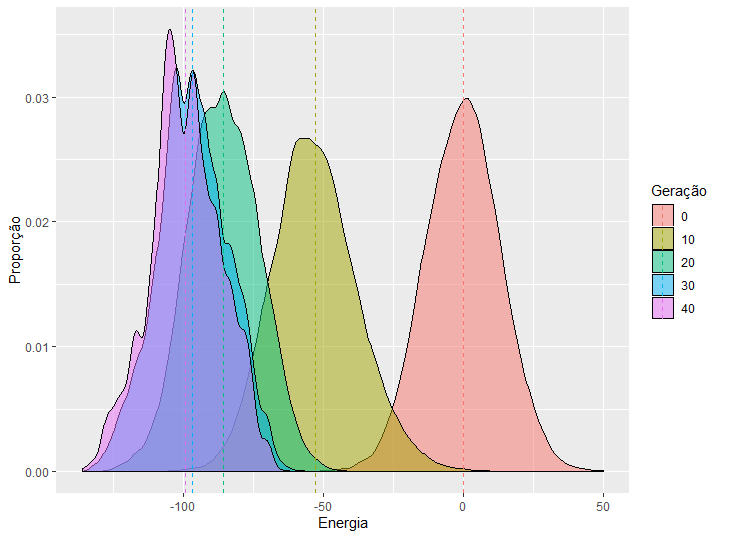
\includegraphics[width=\linewidth]{imagens/Distribuicao_amostral_500_testes_sem_mut.png}
		\caption{Usando amostra dos 500 testes e agrupando por geração}
	\end{subfigure}
\caption{Distribuições das populações para gerações 0, 10, 20 e 40, com \(p_m=0,\)}
	\label{fig:distribuicao_ising_2}
\end{figure}

Na \autoref{fig:distribuicao_ising_geracoes} pode ser visto os resultados das médias e variâncias da população durante as gerações. Os gráficos representam a média das duas medidas de cada geração pelos 500 testes realizados. Quando a taxa de mutação é mantida em 0, percebe-se a rápida convergência do GA, chegando a um patamar mínimo de energia, e a variância com tendência a zero. Ao colocar uma pequena taxa de mutação, o algoritmo converge mais lentamente, porém obtém resultados de média melhores, e a variância se mantém em um patamar. Isso é desejável no GA, pois indica que se manteve a diversidade genética. Além disso também é mostrado novamente o desempenho entre os operadores de crossover de um ponto e uniforme, e como esperado, o uniforme conseguiu médias melhores, mas a variância levou mais iterações para diminuir, justificado pelo fato desse operador obter maior diversidade genética no início, explorando melhor o espaço de soluções e garantindo melhores médias.

\begin{figure}[ht]
	\centering
	\begin{subfigure}[b]{0.47\linewidth}
		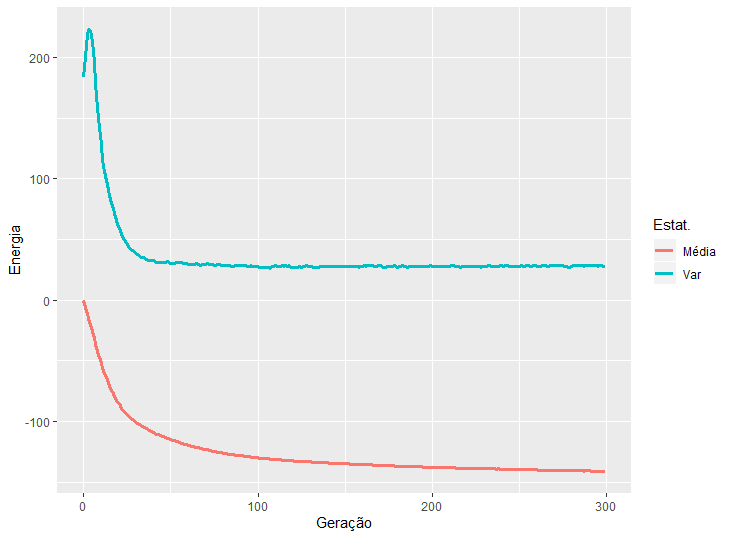
\includegraphics[width=\linewidth]{imagens/curva_media_var_1.png}
		\caption{Usando \(p_m = 0,005\)}
	\end{subfigure}
	\begin{subfigure}[b]{0.47\linewidth}
		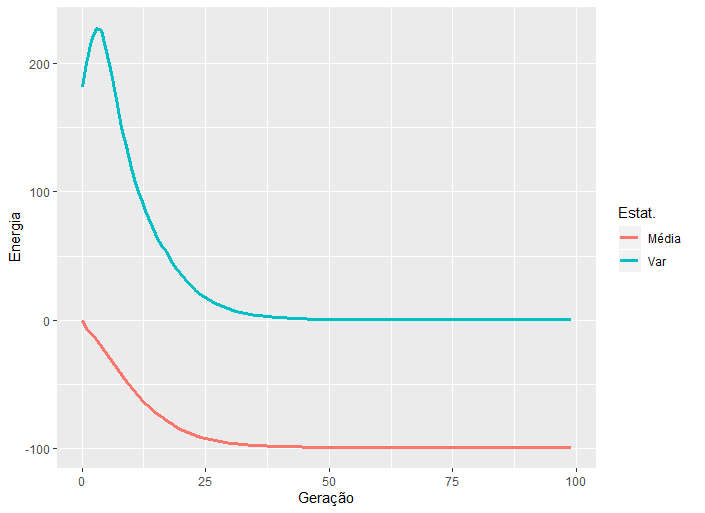
\includegraphics[width=\linewidth]{imagens/curva_media_var_2.png}
		\caption{Usando \(p_m = 0\)}
	\end{subfigure}
	\begin{subfigure}[b]{0.67\linewidth}
		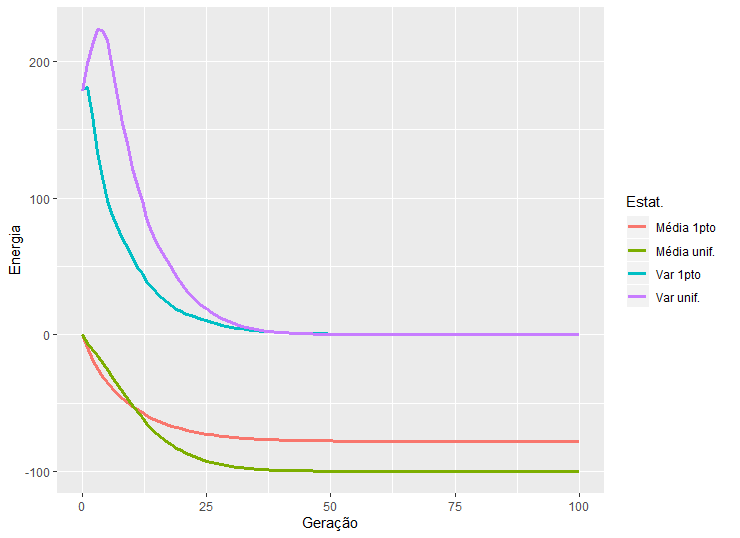
\includegraphics[width=\linewidth]{imagens/comp_cross_1pto_unif.png}
		\caption{Usando \(p_m = 0\) e comparando dois métodos de crossover}
	\end{subfigure}
\caption{Valores das médias e variâncias da população durante as gerações com \(p_m=0,005\). Os valores apresentados são da média de 500 testes}
	\label{fig:distribuicao_ising_geracoes}
\end{figure}

Por último na \autoref{fig:evolucaoGA} é exposto a evolução do algoritmo durante as gerações com variações no parâmetro de probabilidade de mutação, mostrando o melhor, pior cromossomo da população além de sua avaliação média. As linhas horizontais tracejadas mostram o melhor, pior e média do método de busca aleatório, considerando sempre a amostra para esse método de tamanho \(P \cdot T\).

\begin{figure}[ht]
	\centering
	\begin{subfigure}[b]{0.47\linewidth}
		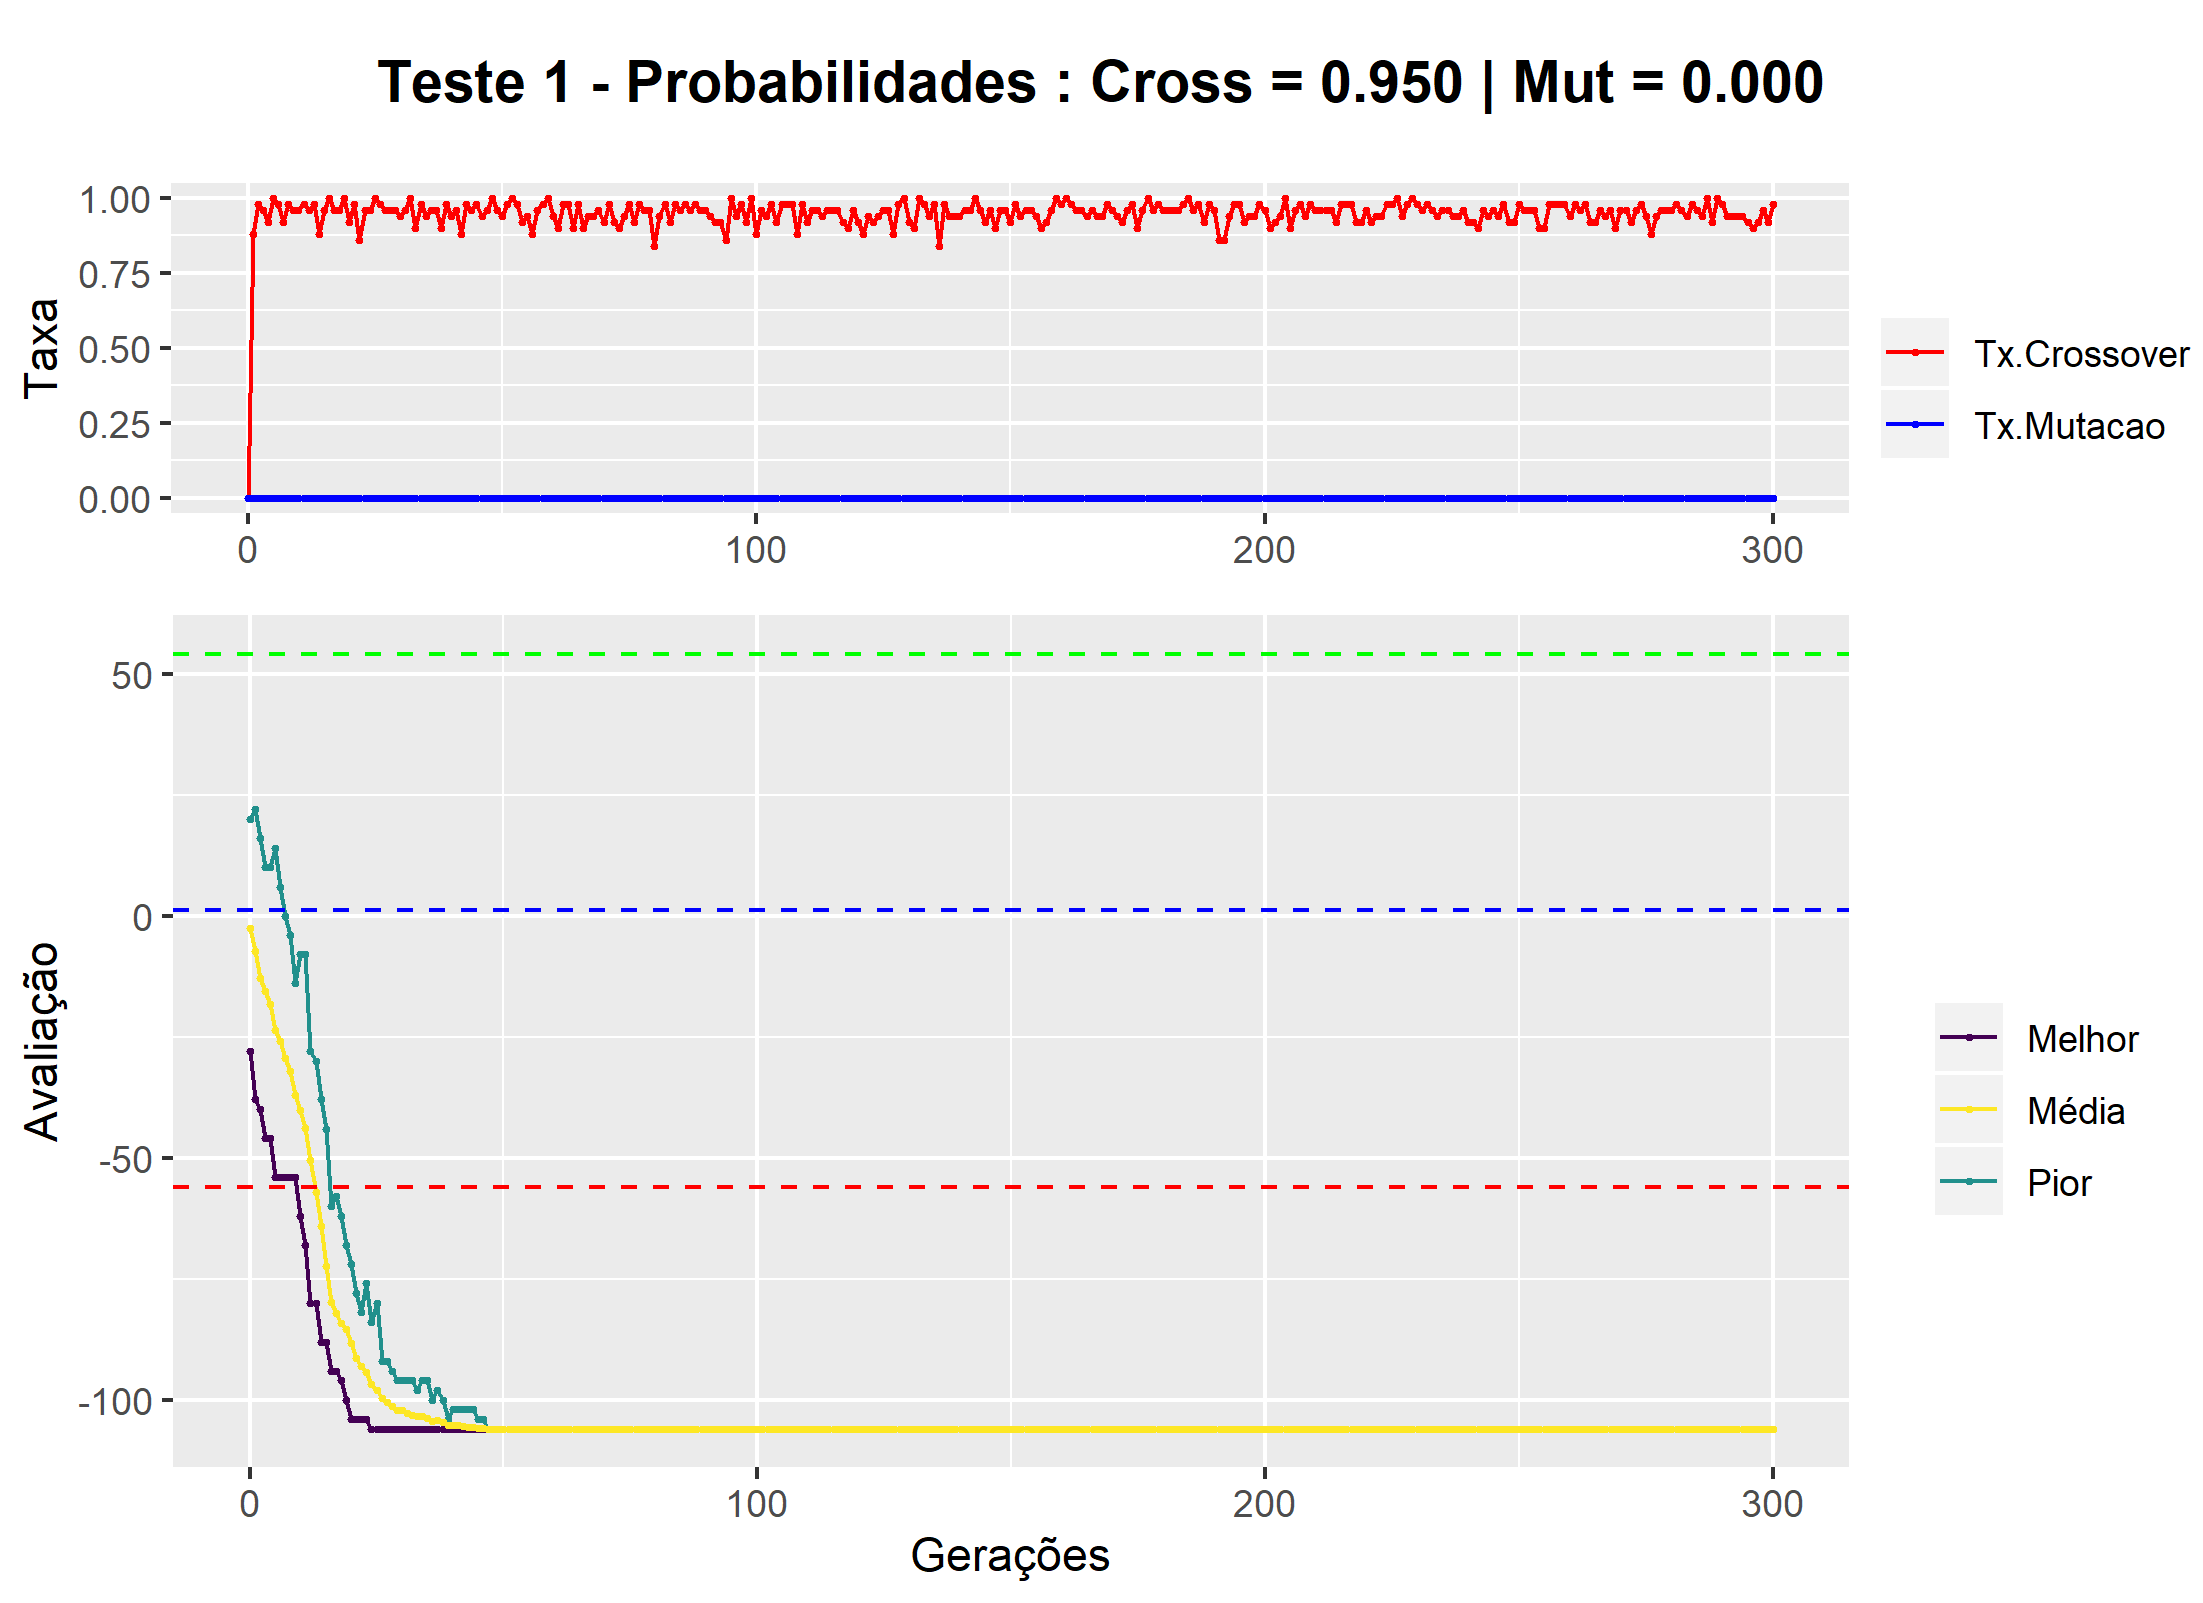
\includegraphics[width=\linewidth]{imagens/graph_pc_0_950_pm_0_000_pop_50_g_300__1.png}
		\caption{}
	\end{subfigure}
	\begin{subfigure}[b]{0.47\linewidth}
		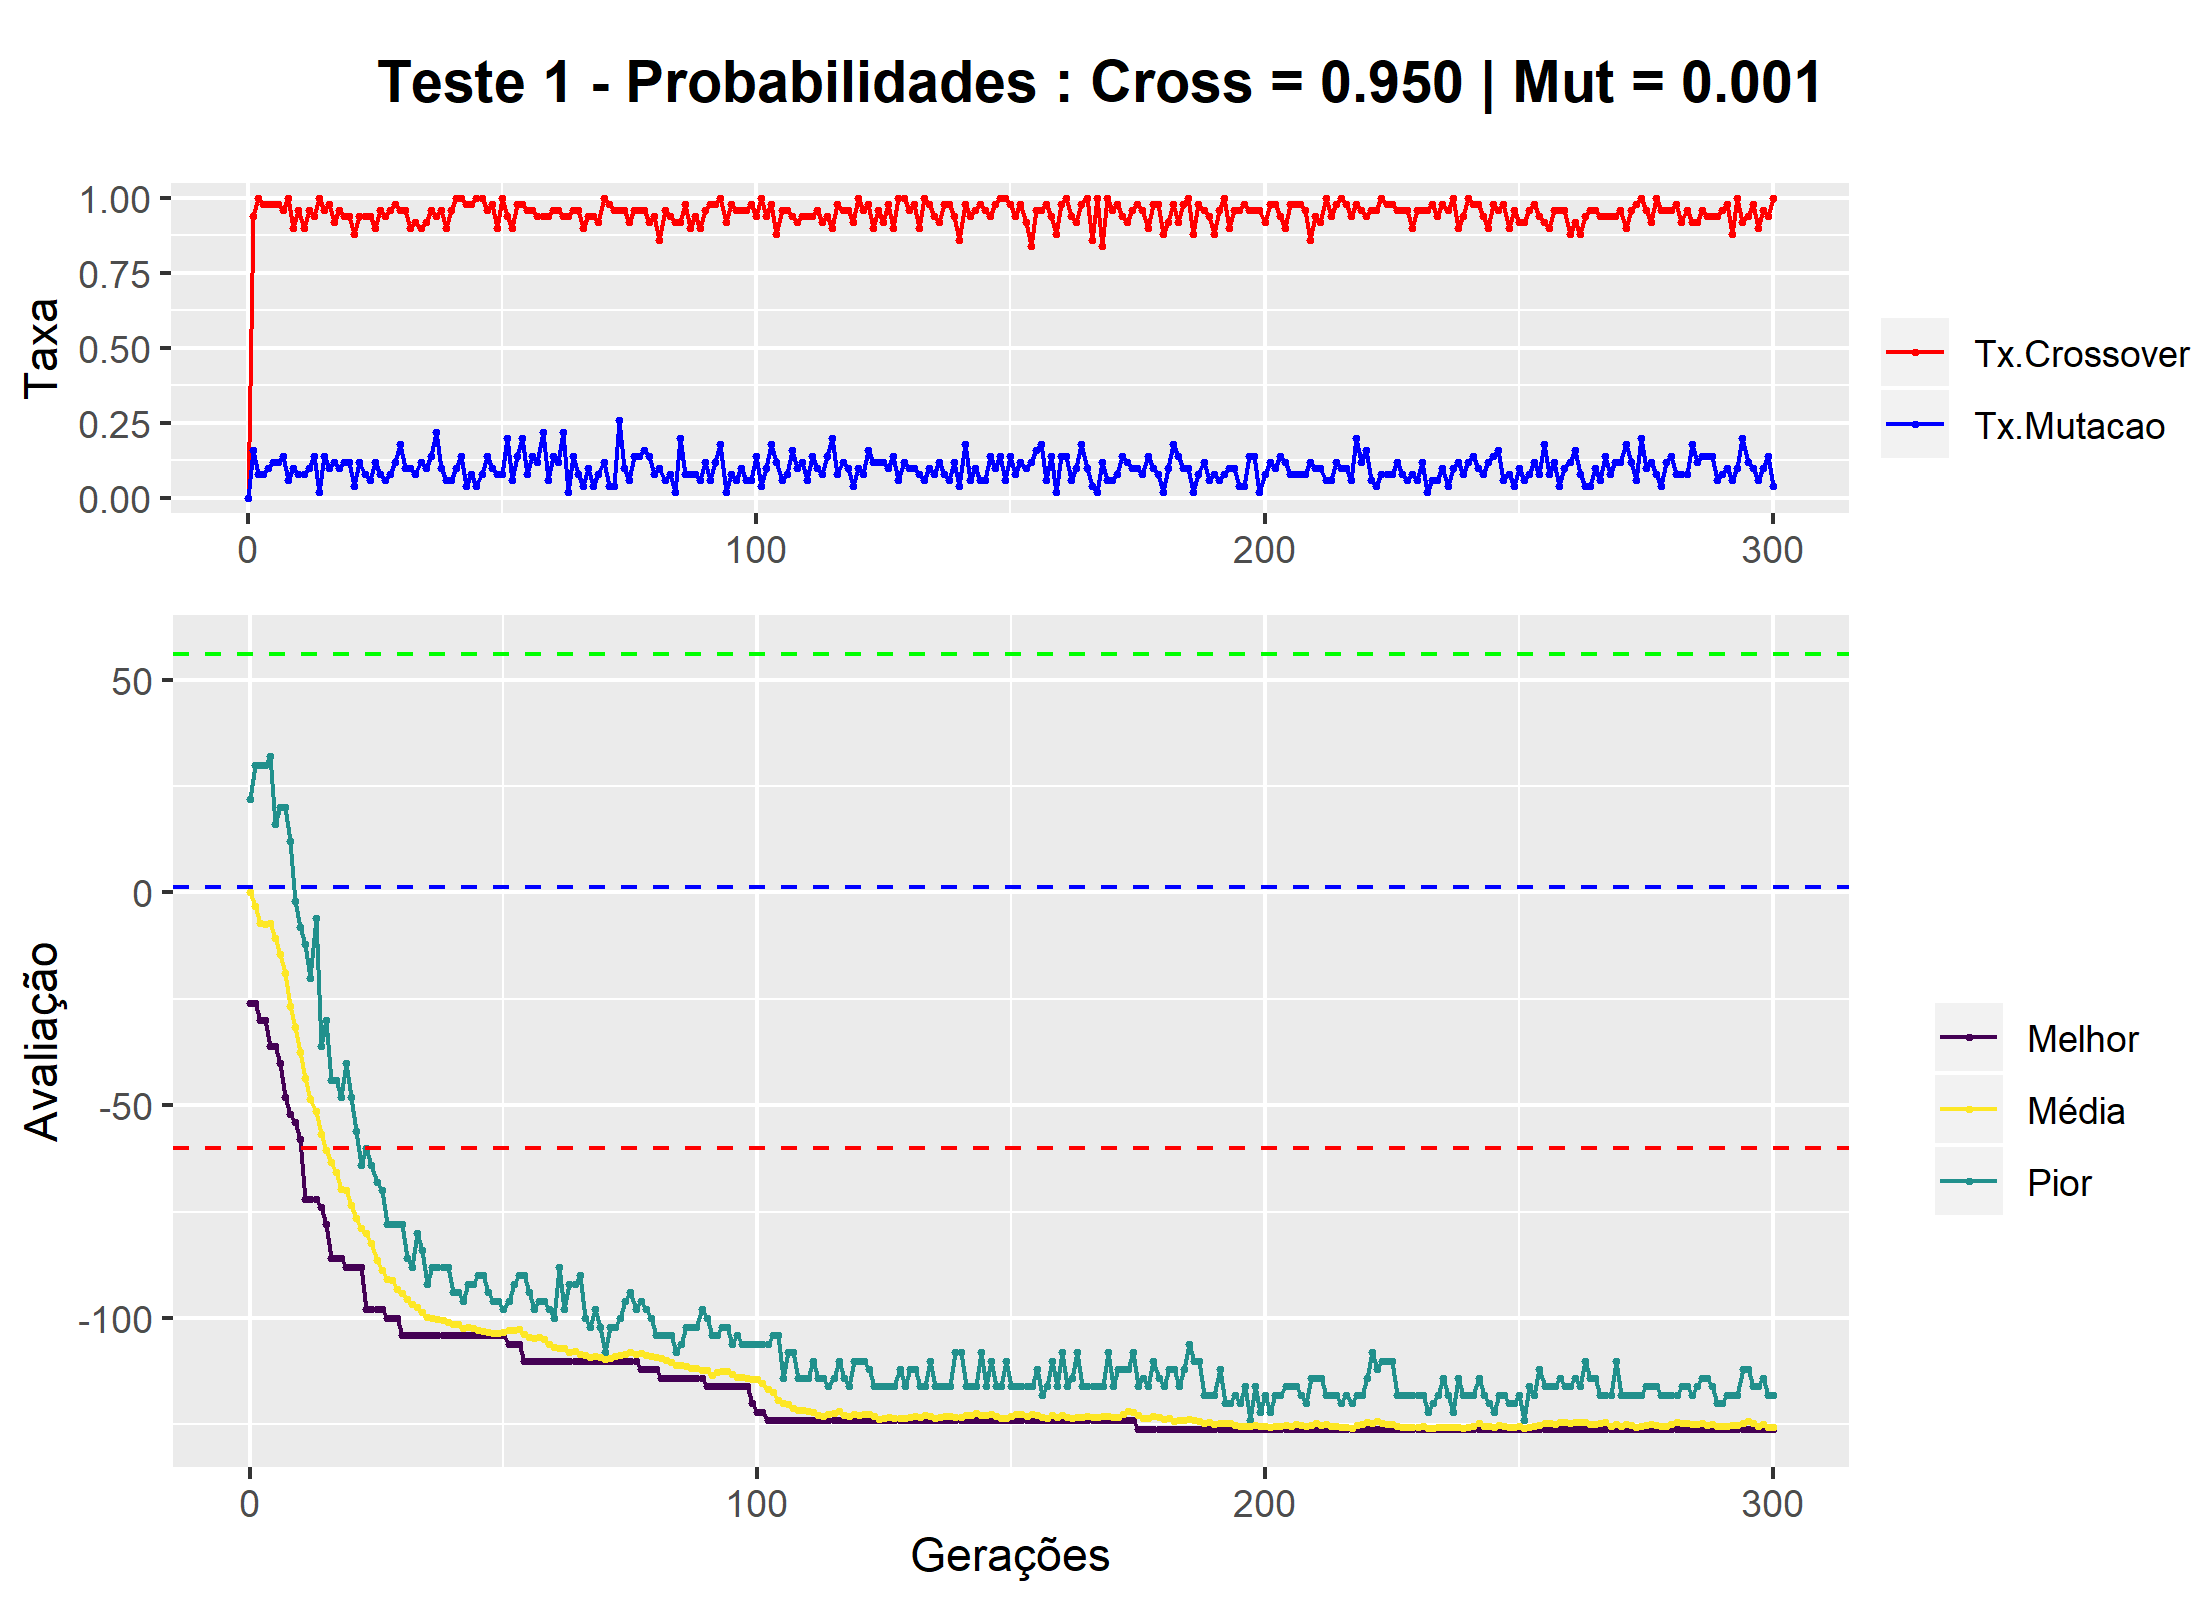
\includegraphics[width=\linewidth]{imagens/graph_pc_0_950_pm_0_001_pop_50_g_300__1.png}
		\caption{}
	\end{subfigure}
	\begin{subfigure}[b]{0.47\linewidth}
		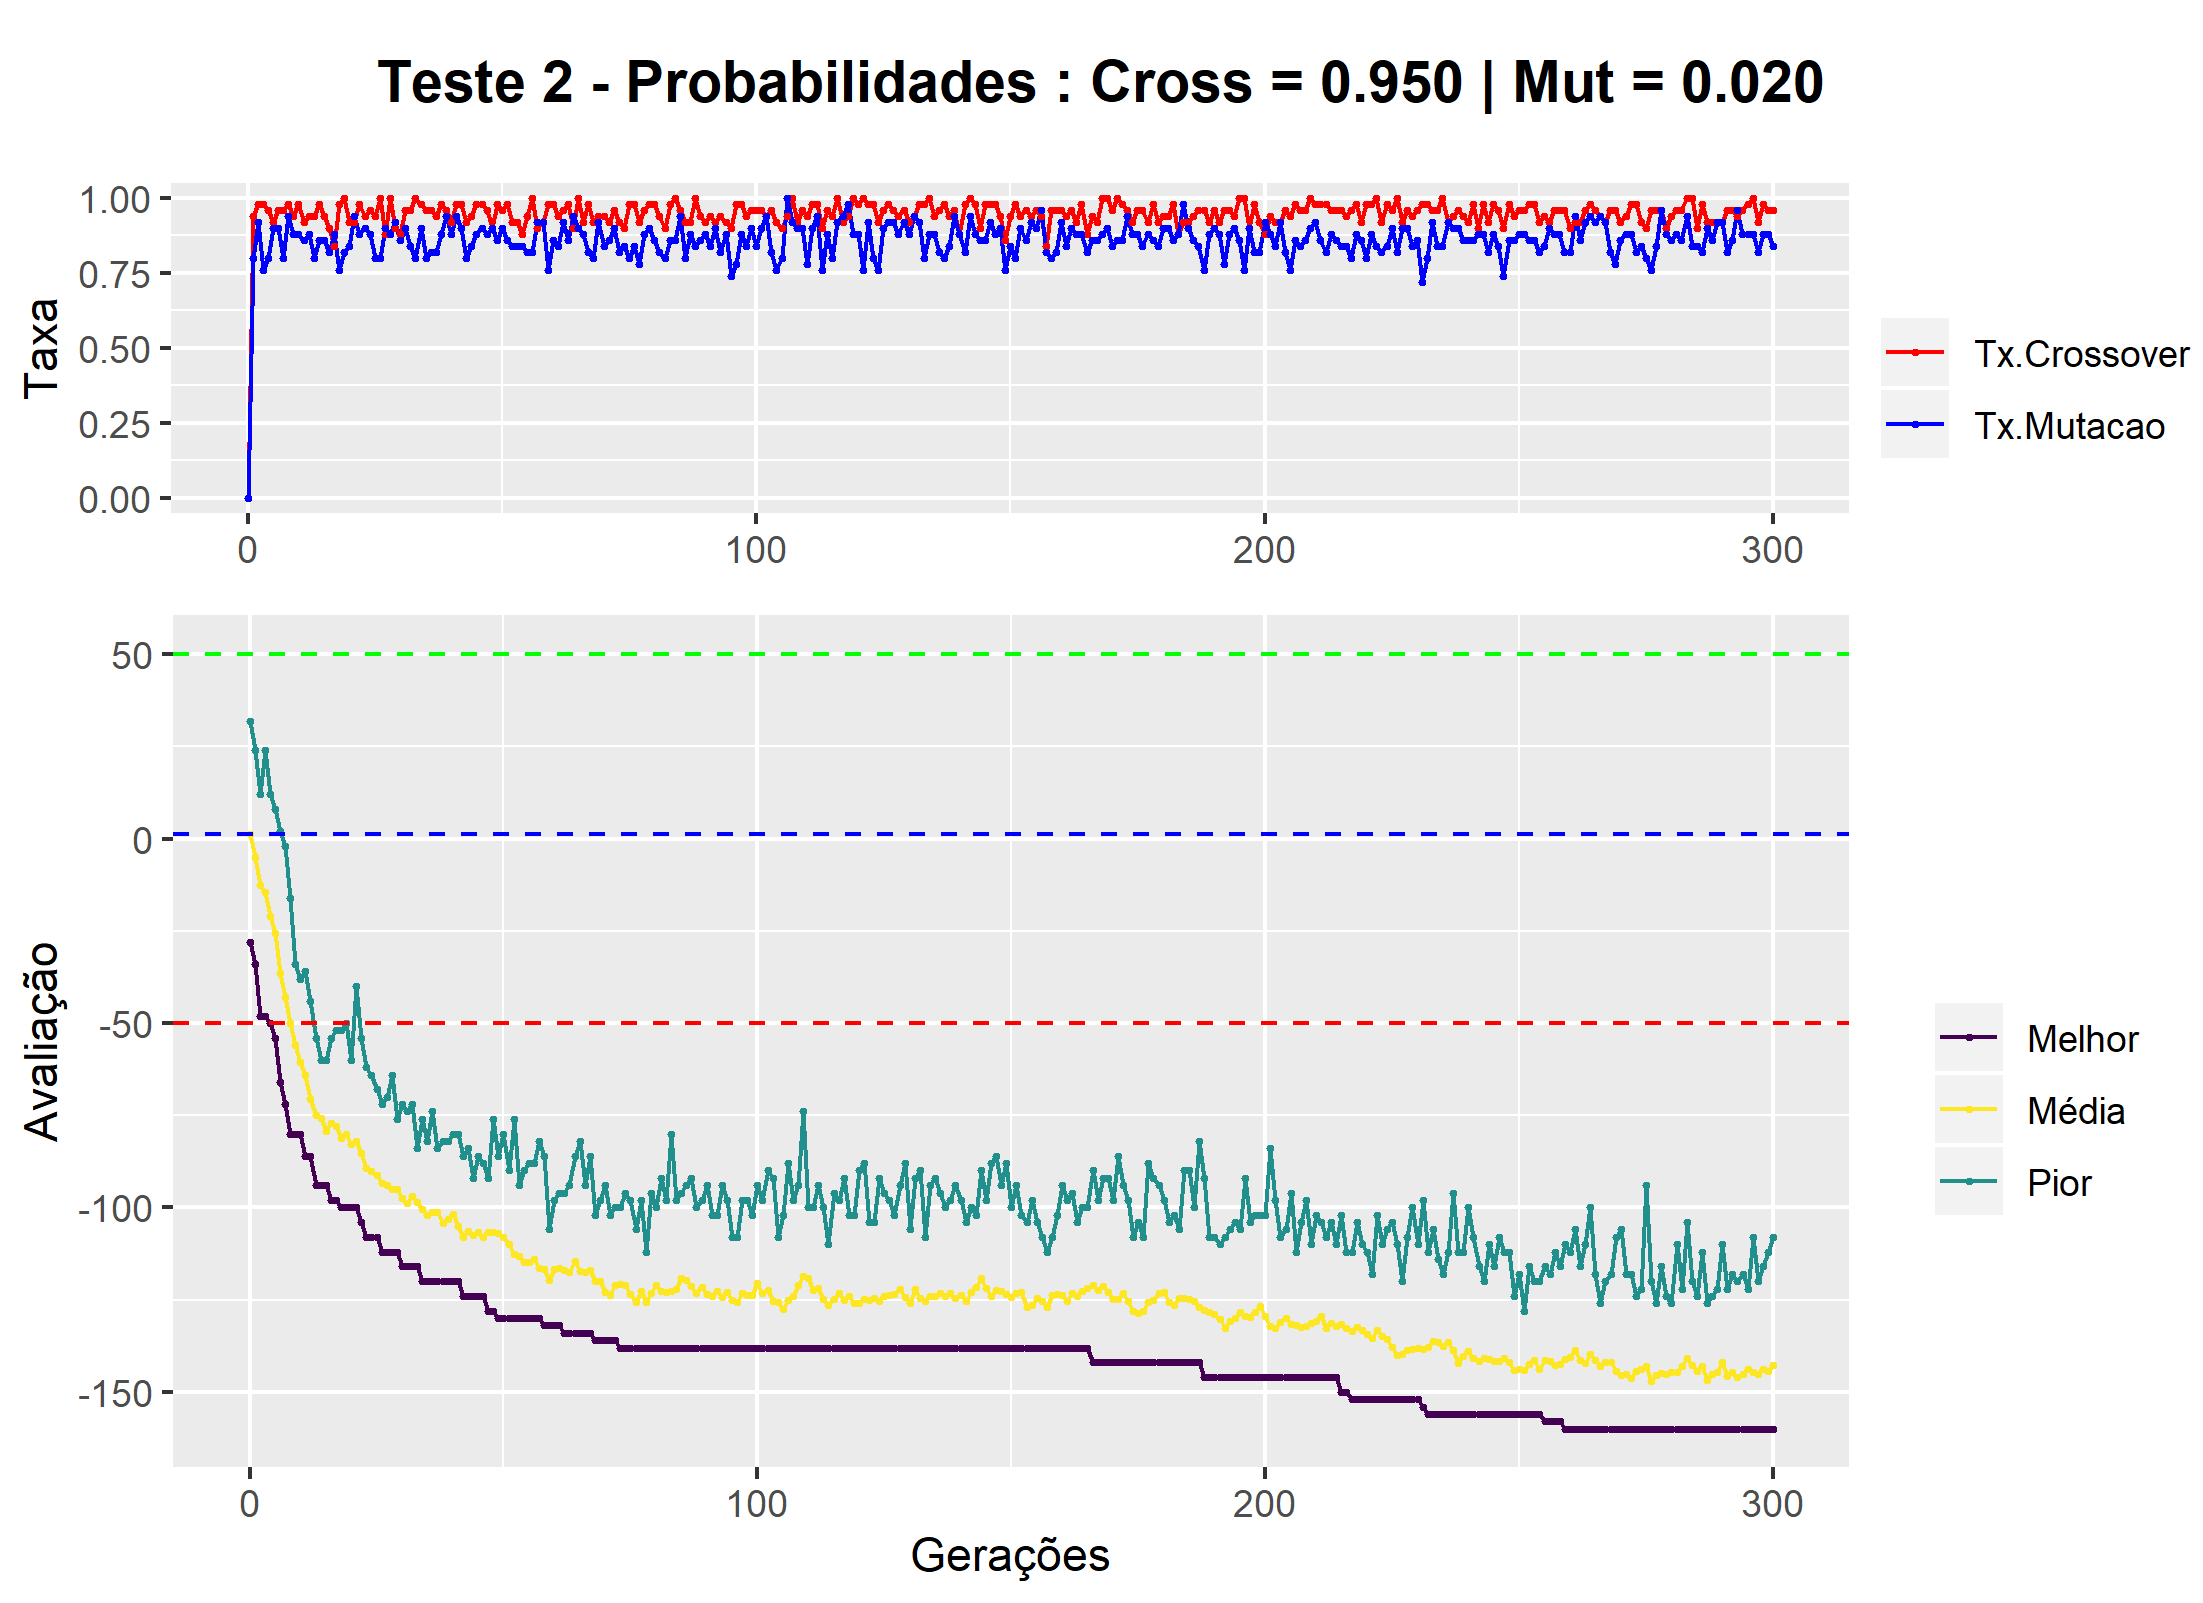
\includegraphics[width=\linewidth]{imagens/graph_pc_0_950_pm_0_020_pop_50_g_300__2.png}
		\caption{}
	\end{subfigure}
	\begin{subfigure}[b]{0.47\linewidth}
		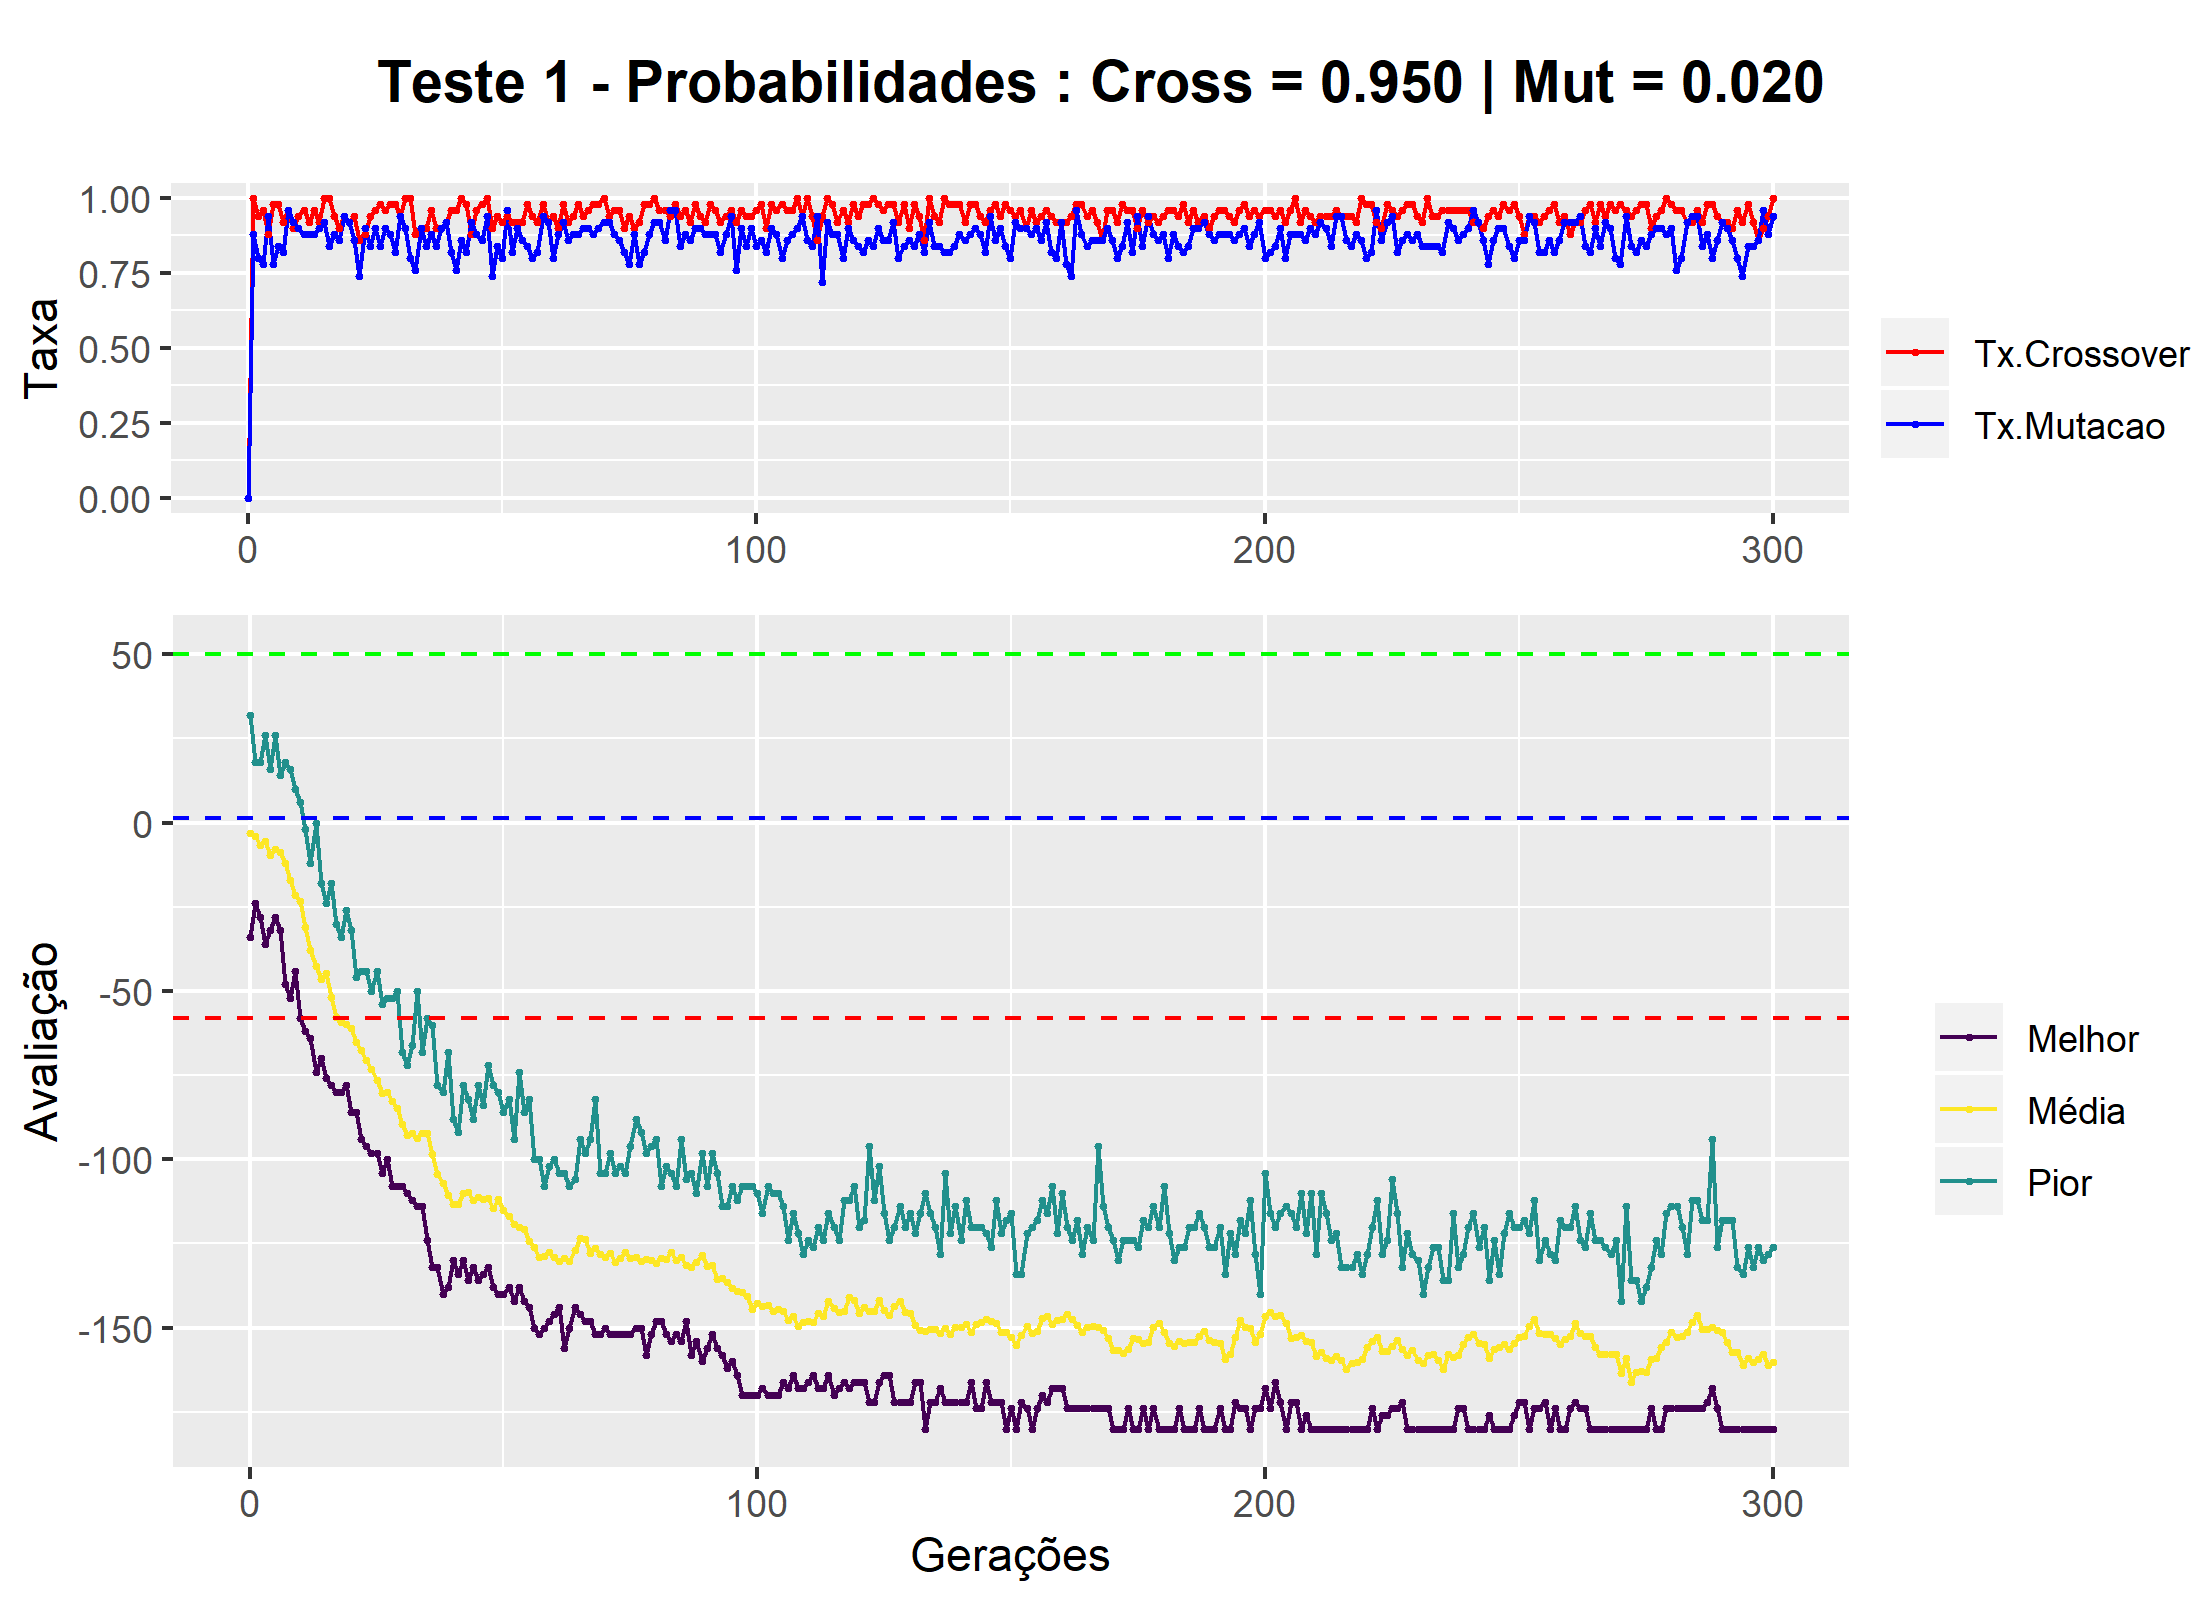
\includegraphics[width=\linewidth]{imagens/graph_pc_0_950_pm_0_020_pop_50_g_300__1_noelite.png}
		\caption{Sem elitismo}
	\end{subfigure}
\caption{Evolução do algoritmo genético durante gerações}
	\label{fig:evolucaoGA}
\end{figure}

Outros gráficos de resultados podem ser vistos na \autoref{fig:evolucaoGA2} do \refanexo{chap:anexos}.